\subsection{Soluciones}

\sol{1}\newline\newline
$a)$ Al ser metálicas, la esfera y el cascarón son conductores.En equilibrio electrostático, la carga en la superficie interior del cascarón es $-q$ para neutralizar el campo eléctrico de la esfera (que no haya líneas de campo en el conductor) y, dado que su carga total es nula, la carga en la superficie exterior es $q$. Las densidades de carga superficial de la esfera $\sigma_S$, interior del cascarón $\sigma_I$ y exterior del cascarón $\sigma_E$ son uniformes, en el caso de $\sigma_I$ porque la esfera y el cascarón son concéntricos, y están dados por

\[\sigma_S = \frac{q}{4\pi R^2}\]
\[\sigma_I = \frac{-q}{4\pi a^2}\]
\[\sigma_E = \frac{q}{4\pi b^2}\]

$b)$ El espacio está dividido en 4 zonas: al interior de la esfera, $r<R$ (1); entre la esfera y el cascarón, $R<r<a$ (2); interior del cascarón, $a<r<b$ (3); y exterior del cascarón, $b<r$ (4). Como el sistema se compone sólo de conductores y vacío, la densidad volumétrica en todo el espacio es nula. Con esto, utilizando la ecuación de Poisson (calculada en \textbf{\ref{PoissonEsferas}}) el potencial dividido en zonas es

\begin{itemize}
    \item $V_1 = B_1 - \frac{A_1}{r}$
    \item $V_2 = B_2 - \frac{A_2}{r}$
    \item $V_3 = B_3 - \frac{A_3}{r}$
    \item $V_4 = B_4 - \frac{A_4}{r}$
\end{itemize}

Para $r\rightarrow\infty$ el potencial se anula, por lo que $B_4 = 0$, además, dado que en los conductores el potencial es constante, $A_1 = A_3 = 0$.

Los campos eléctricos en (2) y (4) poseen simetría de tipo $\Vec{E}(\Vec{r}) = E(r)\hat{r}$ (demostración en \textbf{\ref{SimetríaEsfera}}), de modo que por ley de Gauss se verifica que

\begin{itemize}
    \item $E_2 = \frac{q}{4\pi\epsilon_o r^2}$
    \item $E_4 = \frac{q}{4\pi\epsilon_o r^2}$
\end{itemize}

Utilizando $\Vec{E} = -\nabla V$ se obtiene

\[\frac{q}{4\pi\epsilon_o r^2} = -\frac{A_2}{r^2} = -\frac{A_4}{r^2}\]

\[A_2 = A_4 = -\frac{q}{4\pi\epsilon_o}\]

Finalmente, por continuidad del potencial

\[V_4(b) = V_3(b) \Rightarrow B_3 = \frac{q}{4\pi\epsilon_o b}\]
\[V_3(a) = V_2(a) \Rightarrow B_2 = \frac{q}{4\pi\epsilon_o}
\left(\frac{1}{b}-\frac{1}{a}\right)\]
\[V_2(R) = V_1(R) \Rightarrow B_1 = \frac{q}{4\pi\epsilon_o}
\left(1+\frac{1}{b}-\frac{1}{a}\right)\]

Se concluye así que

\begin{itemize}
    \item $V_1 = \frac{q}{4\pi\epsilon_o}
\left(1+\frac{1}{b}-\frac{1}{a}\right)$
    \item $V_2 = \frac{q}{4\pi\epsilon_o}\left(
    \frac{1}{r}+\frac{1}{b}-\frac{1}{a}\right)$
    \item $V_3 = \frac{q}{4\pi\epsilon_o b}$
    \item $V_4 = \frac{q}{4\pi\epsilon_o r}$
\end{itemize}
\bigbreak

$c)$ Si se baja el potencial del cascarón a 0, en consecuencia el potencial al exterior de este se anula también

\[V_3 = V_4(b) \Leftrightarrow 0 = -\frac{A_4}{b} \Leftrightarrow A_4 = 0	\Leftrightarrow V_4 = 0\]

Si $V_4 = 0$ entonces $E_4= 0$ y, por ley de Gauss, la carga total encerrada por el cascarón en nula, $\sigma_E = 0$. La carga de la esfera no se ve afectada, de modo que $E_2$ y $A_2$ se mantienen iguales, luego

\[V_2(a) = V_3 \Leftrightarrow B_2 = -\frac{q}{4\pi\epsilon_o a}\]
\[V_2(r) = \frac{q}{4\pi\epsilon_o}\left(\frac{1}{r}
-\frac{1}{a}\right)\]
\[V_1 = V_2(R) = \frac{q}{4\pi\epsilon_o}\left(\frac{1}{R}
-\frac{1}{a}\right)\]

\bigbreak

$d)$ Si $V_3 = V$ entonces

\[V_3 = V_4(b) \Leftrightarrow v = -\frac{A_4}{b} \Leftrightarrow A_4 = -Vb	\Leftrightarrow V_4 = \frac{Vb}{r}\]
\[V_2(a) = V_3 \Leftrightarrow B_2 = V-\frac{q}{4\pi\epsilon_o a}
\Leftrightarrow V_2 = V+\frac{q}{4\pi\epsilon_o}\left(\frac{1}{r}
-\frac{1}{a}\right)\]
\[\Vec{E_4}=-\nabla V_4 = \frac{Vb}{r^2}\hat{r}\]

Para $Q$ la carga total, por ley de Gauss se tiene que

\[E_4= \frac{Q}{4\pi\epsilon_o r^2} = \frac{Vb}{r^2}
\Leftrightarrow Q = 4\pi\epsilon_o Vb\]

Por lo que la carga neta del cascarón es

\[q_c = 4\pi\epsilon_o Vb - q\]

\bigbreak

$e)$ Si se conectan la esfera y el cascarón ambos conformarán un solo conductor y por lo tanto estarán a un mismo potencial. Como la diferencia de potencial es nula, el campo eléctrico en todo el espacio encerrado por el cascarón es 0. Dado que no se produce ningún cambio a la carga total, $E_4$, y por ende $V_4$, son los calculados en $b)$

\[V_1=V_2=V_3=V_4(b)=\frac{q}{4\pi\epsilon_o b}\]
\bigbreak

$f)$ La energía de los conductores desconectados es

\[U_{e1} = \frac{1}{2}(qV_1 + 0\cdot V_3) = \frac{q^2}{8\pi\epsilon_o}
\left(1+\frac{1}{b}-\frac{1}{a}\right)\]

Para los conductores conectados la energía es

\[U_{e2} = \frac{1}{2}qV_3 = \frac{q^2}{8\pi\epsilon_o b}\]

Se tiene $U_{e1} > U_{e2}$ debido a que al conectar los cascarones las cargas se desplazan a causa de un trabajo hecho por el campo, causando que la energía en el sistema disminuya.%para $U_{e1}$ a la energía de los conductores se le agrega la de la interacción entre ambos.

\bigbreak
\bigbreak

\sol{2}\newline\newline
Dado que $L \gg R_1, R_2$ el efecto que tiene cada esfera sobre el potencial de la otra puede ser despreciado. Para $q_1$ y $V_1$ la carga y potencial de la esfera de radio $R_1$, y $q_2$ y $V_2$ la carga y potencial de la esfera de radio $R_2$, se tiene

\[V_1 = \int\frac{\sigma_1}{4\pi\epsilon_o R_1}dS = 
\frac{q_1}{4\pi\epsilon_o R_1}\]

\[V_2 = \frac{q_2}{4\pi\epsilon_o R_2}\]

Como están conectadas, el potencial de las esferas debe ser igual

\[V_1 = V_2 \Leftrightarrow \frac{q_1}{R_1} = \frac{q_2}{R_2}\]

luego

\[Q = q_1 + q_2 = q_1 + \frac{R_2}{R_1}q_1 \Leftrightarrow
q_1 = \frac{R_1 Q}{R_1+R_2}\]

\[q_2 = \frac{R_2 Q}{R_1+R_2}\]

Puesto que $R_1<R_2$, la carga almacenada en la esfera de radio $R_2$ es mayor a la de radio $R_1$

\bigbreak

$b)$ El alambre es parte del conductor por lo que

\[V_{alambre} = V_1 = V_2 = \frac{Q}{4\pi\epsilon_o(R_2+R_1)}\]
\bigbreak

$c)$ La densidad de carga de las esferas es

\[\sigma_1 = \frac{q_1}{4\pi R_1^2} =
\frac{Q}{4\pi R_1(R_1+R_2)}\]
\[\sigma_2 = \frac{q_2}{4\pi R_2^2} =
\frac{Q}{4\pi R_2(R_1+R_2)}\]

Como $R_2 > R_1$, $\sigma_2 < \sigma_1$. El campo eléctrico en las superficies es

\[\Vec{E_1}=\frac{\sigma_1}{\epsilon_o}\hat{r_1}\]
\[\Vec{E_2}=\frac{\sigma_2}{\epsilon_o}\hat{r_2}\]

Donde $\hat{r_i}$ es el vector unitario $\hat{r}$ de las coordenadas esféricas respecto al centro de la esfera de radio $R_i$.
\bigbreak
\bigbreak

\sol{3}\newline\newline
 Usando coordenadas esféricas con origen en el centro de las capas, el espacio se divide en 4 zonas: $r < a$ (1), $a<r<2a$ (2), $2a<r<3a$ (3) y $3a<r$ (4). Las esferas presentan simetría (demostración en \textbf{\ref{SimetríaEsfera}}), por lo que se puede calcular su campo eléctrico con ley de Gauss. Como el sistema comprende sólo conductores y vacío $\rho = 0$ en todo el espacio. De la ecuación de Poisson (resuelta en \ref{PoissonEsferas}) se desprende que en cada zona el potencial es de forma
\[V = B-\frac{A}{r}\]


\begin{enumerate}[label=\alph*)]
    \item Como en (1) no hay carga el campo es nulo
    \[E_1 = 0\]
    \item En (2) la carga encerrada es $Q_{in}$, por lo que el campo eléctrico es
    \[\Vec{E_2} = \frac{Q_{in}}{4\pi\epsilon_o r^2}\hat{r}\]
    \item En (3) la carga encerrada es $Q_{in}+Q$, por lo que el campo eléctrico es
    \[\Vec{E_2} = \frac{Q_{in}+Q}{4\pi\epsilon_o r^2}\hat{r}\]
    \item Para que no haya campo eléctrico al interior del conductor exterior se debe cumplir que $Q_{out} = -(Q+Q_{in})$. Como en el infinito el potencial se anula, en (4) $B=0$ y $V = -\frac{A}{r}$. Igualando $V$ a 0 en $3a$ se obtiene que $A=V=0$ y en concecuencia
    \[E_4 = 0\]


    \item Para $V_2$ el potencial en (2), se verifica que

    \begin{equation}
    \begin{split}
        V_2(r) & = V_2(r) - V_2(a)\\
        & = -\int^r_a\Vec{E_2}\cdot d\Vec{r'}\\
       & = -\int^r_a\frac{Q_{in}}{4\pi\epsilon_o {r'}^2}\,dr'\\
       & = \frac{Q_{in}}{4\pi\epsilon_o r} - \frac{Q_{in}}{4\pi\epsilon_o a}\\
    \end{split}
    \nonumber
    \end{equation}
    Con lo que el potencial en la capa intermedia es

    \[V_2(2a) = -\frac{Q_{in}}{8\pi\epsilon_o a}\]
    \medbreak
    Para $V_3$ el potencial en (3), se verifica que

    \begin{equation}
    \begin{split}
      V_3(r) & = V_3(r) - V_3(3a)\\
      & = -\int^r_{3a}\Vec{E_3}\cdot d\Vec{r'}\\
      & = -\int^r_{3a}\frac{Q_{in}+Q}{4\pi\epsilon_o {r'}^2}\,dr'\\
      & = \frac{Q_{in}+Q}{4\pi\epsilon_o r} - \frac{Q_{in}+Q}{12\pi\epsilon_o a}\\
    \end{split}
    \nonumber
    \end{equation}
    Con lo que el potencial en la capa intermedia es

    \[V_3(2a) = \frac{Q_{in}+Q}{24\pi\epsilon_o a}\]
    \medbreak
    \item Como $V_2(2a)=V_3(2a)$, se tiene que

    \[\frac{Q_{in}+Q}{24\pi\epsilon_o a} = -\frac{Q_{in}}{8\pi\epsilon_o a}\]
    \[\implies Q_{in}=-\frac{1}{4}Q\]
    
    \medbreak
    \item Puesto que las capas exterior e interior están a igual potencial se las puede tomar como un solo conductor de carga $Q_{in} + Q_{out} = -Q$, formando un condensador con la capa intermedia. La capacitancia del sistema está dada por
    
    
    \[C = \frac{Q}{\Delta V} = 32\pi\epsilon_o a\]
    
    Esto también se puede ver como si se tuvieran dos condensadores en paralelo, uno con carga $Q_{in}$ y otro con carga $Q_{out}$ y misma diferencia de potencial $V(2a)$. Al estar en paralelos su capacitancia equivalente sería la suma de las capacitancias individuales, dando el resultado anterior.
    
    La razón de que pueden verse como condensadores en paralelo yace en que poseen el mismo potencial en ambos extremos, en uno están a potencial $V=0$ y en el otro a potencial $V = V(2a)$. En la siguiente imagen se visualiza de manera circuital
    
    \begin{figure}[H]
        \centering
        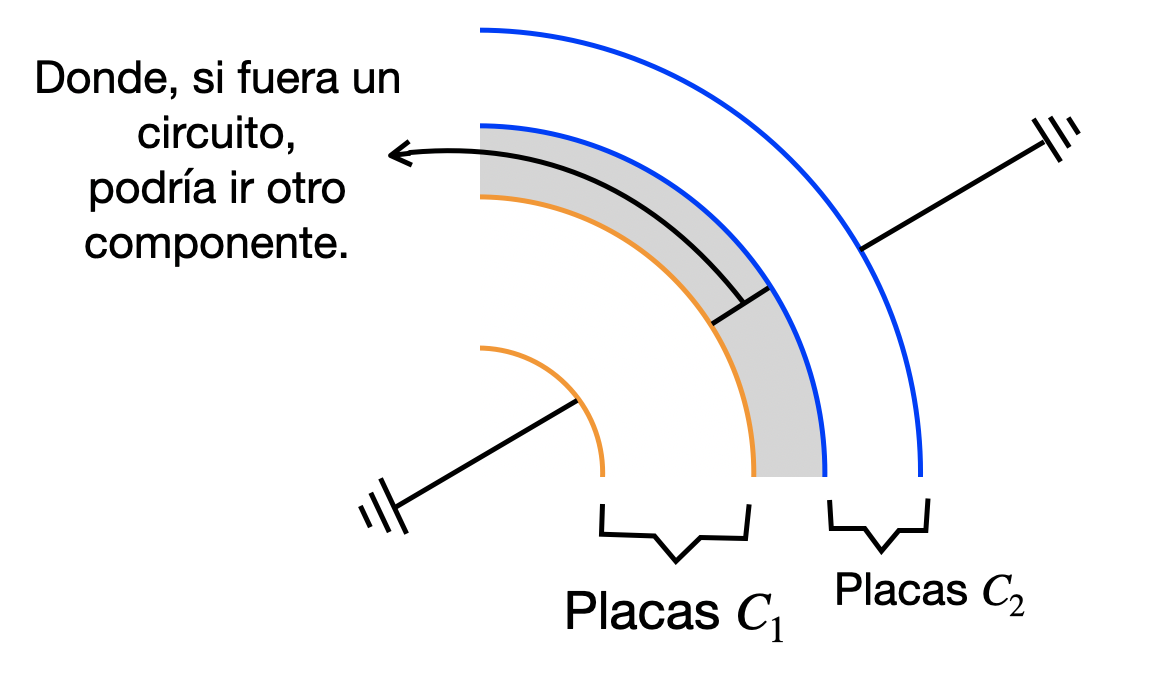
\includegraphics[width=0.5\textwidth]{Electroestática/conductores/P3IG.png}
    \end{figure}
    
    En la figura anterior el conductor de radio $a$ es el inferior izquierdo, el conductor de radio $2a$ está representado por el conductor 'con anchura' de color gris, y el conductor de radio $3a$ es el superior derecho. Las conexiones con 3 líneas representan conexiones a tierra. Y los condensadores son representados el primero con color amarillo-naranjo y el segundo con color azul. 
    
    \medbreak
    \item El sistema está compuesto por 3 conductores y 2 condensadores, como las capas interna y externa tienen potencial nulo, la energía queda dada sólo por la capa intermedia

    \[U_e = \frac{1}{2}V_2(2a) = \frac{1}{8}\frac{Q^2}{8\pi\epsilon_o a}\]
    
    Esto es equivalente a calcular la capacitancia de un condensador equivalente y, haciendo uso de $V(2a)$, obtener la energía potencial con
    $U_e = \frac{1}{2}C\Delta V^2$. 

\end{enumerate}
\bigbreak
\bigbreak
\sol{4}\newline
% Podriamos especificar la alineación de las placas y agregar imagen

\begin{enumerate}[label=\alph*)]
    %a
    \item Como las dimensiones laterales de las placas son mucho más grandes que $x$, se puede aproximar el campo eléctrico de una de las placas al de un plano infinito

    \[\Vec{E} = \frac{Q}{2A\epsilon_o}\hat{x}\]

    ubicando el origen en la placa de carga $Q$, el trabajo par desplazar la placa de carga $-Q$ en $\Delta x$ es

    \begin{equation}
        \begin{split}
            W_{ext} &= Q\int^{x+\Delta x}_x \Vec{E}\cdot d\Vec{r}\\
            & = Q\int^{x+\Delta x}_x\frac{Q}{2A\epsilon_o}\,dr\\
            & = \frac{Q^2}{2A\epsilon_o}\Delta x\\
        \end{split}
        \nonumber
    \end{equation}
    \medbreak
%b
    \item Por teorema de trabajo-energía, se cumple que la diferencia de energía potencial es igual al trabajo hecho por la fuerza externa, por lo que

    \[\Delta U_e = W = \frac{Q^2}{2A\epsilon_o}\Delta x\]
    Notemos que al ser el trabajo positivo, la fuerza externa está inyectando energía al sistema, por lo que se tiene que no se conserva la energía del sistema al aumentar la separación entre las placas por un $\Delta x$
    
    La energía potencial del sistema también se puede calcular haciendo uso del condensador, donde $U_e = \frac{1}{2}Q\Delta V = \frac{Q^2}{2C}$. Como se tiene que la carga de las placas no cambia, entonces se tiene que $C$ y $\Delta V$ han de cambiar. En específico, como se separan las placas $C$ pasa a ser $\frac{\epsilon_o A}{x+\Delta x}$ (calculado en \ref{C:placas}).
%c Aux_5 Daniela Mancilla Otoño 2020
    \item Siguiendo la idea del párrafo anterior, si es que al realizar trabajo cambia la energía del sistema, lo que implica un cambio en el condensador, (carga o diferencia de potencial) entonces al mantener la batería conectada se mantendrá la diferencia de potencial igual. Con esto en mente, entonces será necesario que la carga del condensador cambie.
    
    \begin{equation}
    \begin{split}
        W_{ext} &= \int^{x+\Delta x}_x Q\Vec{E}\cdot d\Vec{r}\\
        & = \int^{x+\Delta x}_x \frac{Q^2}{2A\epsilon_o}\,dr\\
        & = \int^{x+\Delta x}_x
        \frac{(CV_o)^2}{2A\epsilon_o}\,dr\\
        & = \int^{x+\Delta x}_x
        \frac{\epsilon_o AV_o^2}{2r^2}\,dr\\
        &=\frac{\epsilon_o AV_o^2}{2}\left(
        -\frac{1}{x+\Delta x}+\frac{1}{x}\right)\\
        &=\frac{\epsilon_o AV_o^2\Delta x}{2x(x+\Delta x)}
    \end{split}
    \nonumber
    \end{equation} 
    
    \medbreak

%d
    \item La energía potencial eléctrica inicial es
    
    \[U_i = \frac{1}{2}C_iV_o^2 = \frac{\epsilon_o A}{2x}V_o^2\]
    
    la energía potencial final es
    
    \[U_f = \frac{1}{2}C_fV_o^2 = 
    \frac{\epsilon_o A}{2(x+\Delta x)}V_o^2\]
    
    de modo que
    
    \[\Delta U = U_f-U_i = -\frac{\epsilon_o AV_o^2\Delta x}{2x(x+\Delta x)}\]
    
    % Hay que mostrar que la energía que se conserva

\end{enumerate}

\bigbreak
\bigbreak

\sol{5}\newline

\begin{enumerate}[label=\alph*)]
    \item El campo eléctrico en todo el espacio puede ser obtenido haciendo uso de la Ley de Gauss y de la definición de campo eléctrico, debido a lo que será pedido en los siguientes incisos solo será calculado en el caso $\rho > a$ y $\abs{z} < L/2$. Donde se están usando coordenadas cilíndricas y el centro del cilindro como eje.\\
    
    Partamos calculando la densidad superficial de carga, la densidad de carga es superficial a causa de que estamos frente a un conductor que no puede tener campo eléctrico interno, con esto tenemos que 
    \[\sigma = \frac{Q}{2\pi aL}\]
    A causa de que está solo en el manto y el área del manto es $2\pi aL$.\\
    
    Haciendo uso de la Ley de Gauss y sabiendo que por simetría (\ref{SimetríaCilindrosInf}) hay solo campo en la dirección $\hat{\rho}$, establecemos un cilindro más grande superpuesto con el original, de radio $\rho$ y altura $h$, con esto
    %no tiene que ser infinito?, no también el largo(altura) puede ser mucha mayor al radio
    \begin{equation}
        \begin{split}
            &\oint_{Manto} \Vec{E}\cdot d\Vec{S} = \frac{Q_{enc}}{\epsilon_0}\\
            \implies &\int E(\rho)dS = \frac{\sigma 2\pi a h}{\epsilon_0}\\
            \implies &E(\rho) \int dS = \frac{\sigma 2\pi a h}{\epsilon_0}\\
            \implies &E(\rho) 2 \pi \rho h = \frac{\sigma 2\pi a h}{\epsilon_0}\\
            \implies &E(\rho) = \frac{\sigma a}{\epsilon_0 \rho}\\
            \therefore \quad &\Vec{E}(\rho) = \frac{\sigma a}{\epsilon_0 \rho}\hat{\rho}
        \end{split}
        \nonumber 
    \end{equation}
    
    \item Sea $\sigma_+$ la densidad superficial del manto del cilindro de radio $a_1$ y $\sigma_-$ la densidad superficial del manto del cilindro de radio $a_2$, tenemos que el campo eléctrico de cada cilindro será
    
    \[\Vec{E}_{a_1} = \frac{\sigma_+ a_1}{\epsilon_0 \rho}\hat{\rho}\]
    \[\Vec{E}_{a_2} = \frac{\sigma_- a_2}{\epsilon_0 \rho}\hat{\rho'}\]
    
    Si calculamos el campo en $P$ debemos sumar ambos campos, y se tiene que $\hat{\rho'} = - \hat{\rho}$, ya que están centrados en distintos ejes los campos, y en $P$ las direcciones son justo contrarias, así
    
    \[\Vec{E}_{\text{en P}} = \left( \frac{\sigma_+ a_1}{\epsilon_0 r} - \frac{\sigma_- a_2}{\epsilon_0 (d-r)} \right)\hat{\rho}\]
    
    \item Para calcular la diferencia de potencial calculamos $V(a_1) - V(d - a_2)$ por definición,
    
    \begin{equation}
        \begin{split}
            V(a_1) - V(d - a_2) &= -\int_{d-a_2}^{a_1}\left[ \frac{\sigma_+ a_1}{\epsilon_0 r} - \frac{\sigma_- a_2}{\epsilon_0 (d-r)} \right]dr\\
            &= -\left.\left[ \frac{\sigma_+ a_1}{\epsilon_0}\ln{(r)} + \frac{\sigma_- a_2}{\epsilon_0}\ln{(d-r)} \right]\right\rvert_{d-a_2}^{a_1}\\
            &\vdots \quad\\ 
            &\approx -\left[ \frac{\sigma_+}{\epsilon_0}a_1\ln{\left( \frac{a_1}{d} \right)} - \frac{\sigma_-}{\epsilon_0}a_2\ln{\left( \frac{a_2}{d} \right)} \right]\\
            \text{Donde en } \vdots \text{ se usó que } &d-a_1 \approx d\text{ y } d-a_2 \approx d\text{, al ser }d \gg a_1\text{ y } d \gg a_2\\
        \end{split}
        \nonumber
    \end{equation}
    
    Reemplazamos $\sigma_+ = Q/(2\pi La_1)$ y $\sigma_- = -Q/(2\pi La_2)$, y nos queda
    
    \begin{equation}
        \begin{split}
            \Delta V &= -\left[ \frac{Q}{2 \pi L\epsilon_0}\ln{\left( \frac{a_1}{d} \right)} + \frac{Q}{2 \pi L\epsilon_0}\ln{\left( \frac{a_2}{d} \right)} \right]\\
            &=\frac{Q}{2 \pi L \epsilon_0}\ln{\left( \frac{d^2}{a_1a_2} \right)}\\
            &=\frac{Q}{\pi L \epsilon_0}\ln{\left( \frac{d}{\sqrt{a_1a_2}} \right)}
        \end{split}
        \nonumber
    \end{equation}
    
    Lo que nos da que la capacitancia del sistema es
    \[C_{tot} \approx \frac{Q}{\Delta V} = \frac{\pi \epsilon_0 L}{\ln{\left( \frac{d}{\sqrt{a_1a_2}} \right)}}\]
    
    \item Como se tiene que nos piden la capacitancia por unidad de largo debemos dividir la capacitancia encontrada por $L$, así
    \[C \approx \frac{\pi \epsilon_0}{\ln{\left( \frac{d}{\sqrt{a_1a_2}} \right)}}\]
    
    \item Está situación es similar a la presentada en el problema 7.2, por lo que las cargas se distribuirían a través de los cilindros dependiendo de las razones entre sus radios, y el potencial se volvería el mismo para ambos.
    
\end{enumerate}

\sol{6}\newline

\begin{enumerate}[label=\alph*)]
    \item Digamos que la capa del radio interno tiene una carga $-Q$ en su cara exterior, y la capa externa una carga $Q$ en su cara interior. Así queda la configuración como en la siguiente imagen
    \begin{figure}[H]
        \centering
        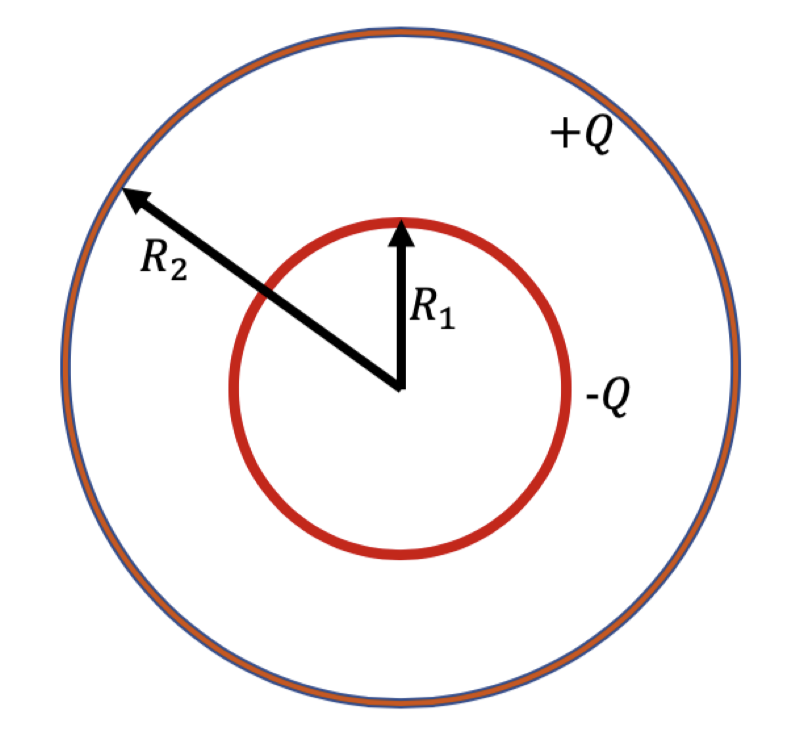
\includegraphics[width=0.47\textwidth]{Electroestática/conductores/P6IA.png}
        \label{fig:sol_6_conduc}
    \end{figure}
    
    Para calcular la capacitancia calculemos la diferencia de potencial entre ambas caras, para esto calculemos el campo eléctrico e integramos de $R_1$ a $R_2$.\\
    
    Usando Ley de Gauss y una superficie Gaussiana de largo $L$ y radio $\rho$, con $R_1 < \rho < R_2$,
    \[\oint_{Manto} \Vec{E}\cdot d\Vec{S} = \frac{Q_{enc}}{\epsilon_0}\]
    \[\implies E(\rho) = \frac{-Q}{2 \pi L \epsilon_0 \rho}\]
    Ahora calculamos la diferencia de potencial,
    \[\Delta V = V(R_2) - V(R_1) =-\int_{R_1}^{R_2}\frac{-Q}{2 \pi L \epsilon_0 \rho}d\rho = \frac{Q}{2\pi L \epsilon_0}\ln{\left( \frac{R_2}{R_1} \right)}\]
    Ahora usando $C = Q/\Delta V$ podemos obtener la capacitancia del sistema
    \[C = \frac{Q}{\Delta V} = \frac{2\pi L \epsilon_0}{\ln{\left( \frac{R_2}{R_1} \right)}}\]
    \text{ }\\     
    % Problema 2 Aux 5 D. Mancilla Otoño2020 (Pauta en Ucursos)
    
    \item \textbf{(Sin valores actualmente)} El nuevo condensador es como el mostrado a continuación
    \begin{figure}[H]
        \centering
        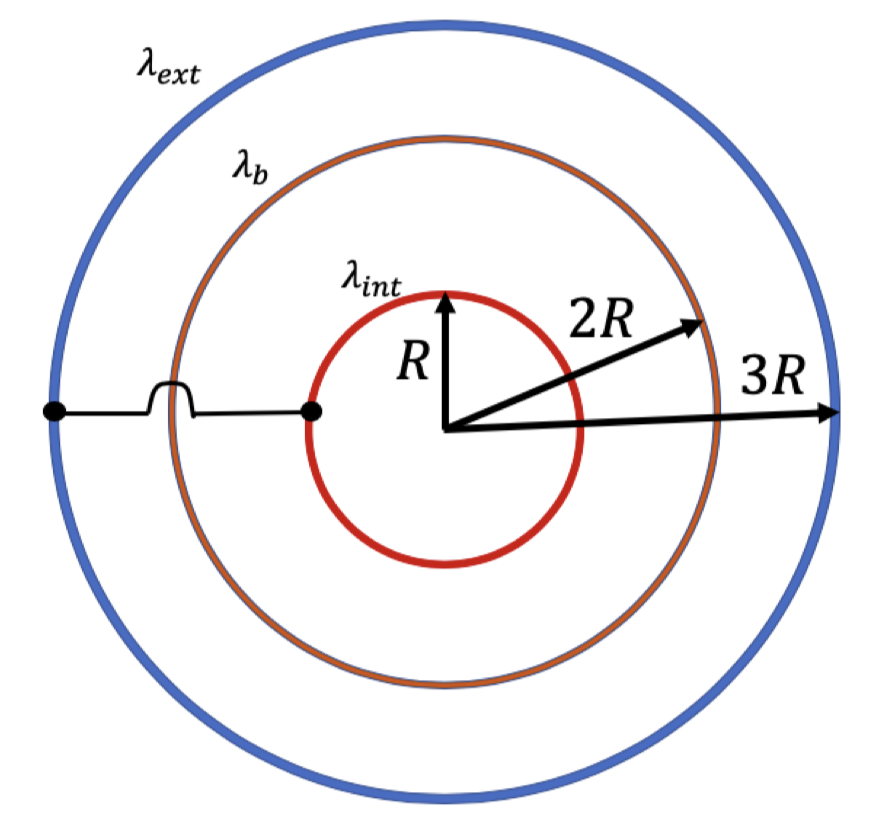
\includegraphics[width=0.47\textwidth]{Electroestática/conductores/P6IB.png}
    \end{figure}
    % Completar respuestas con desarrollo y resultados
    Como se tiene que la capa de radio $R$ y la de radio $3R$ están conectadas entonces sus potenciales son iguales, sabiendo esto y con la Ley de Gauss se puede calcular el campo eléctrico y obtener expresiones para los voltajes. Y usando $V(R) - V(2R) = V(3R) - V(2R)$ se puede despejar $\lambda_{int}$. Luego usando que son conductores y comienzan neutrales se tiene $0 = \lambda_{ext} + \lambda_{int} + \lambda_b$, y se puede obtener el valor de $\lambda_{ext}$
    % Completar respuestas con desarrollo y resultados    
    \item Para despejar la capacitancia se ocupa la relación entre energía potencial eléctrica y capacitancia, y además se despeja usando la definición que la relaciona con el voltaje.
    % (Copiado del aux)
    \item Las cargas ($\lambda_{int}, \lambda_{ext} $ y $ \lambda_b$) permanecen donde se encontraban. Con respecto a $\lambda_{nuevo}$, se distribuirá de manera uniforme en la superficie exterior ($r=3R$).
    
    
\end{enumerate}
\newpage